\documentclass[nojss]{jss}
\usepackage{amsfonts,thumbpdf}

\newtheorem{lemma}{Lemma}
\newtheorem{theorem}{Theorem}
\newtheorem{corollary}{Corollary}
\newtheorem{example}{Example}
\newtheorem{proposition}{Proposition}
\newtheorem{definition}{Definition}
\newtheorem{conjecture}{Conjecture}
\newtheorem{assumption}{Assumption}
\def\logit{\mathop{\rm logit\,}\nolimits}
\def\midd{\mathop{\,|\,}\nolimits}
\def\defn{{\stackrel{\rm def}{=}}}
\def\eqdistn{{\stackrel{\cal D}{=}}}
\newcommand{\bea}{\begin{eqnarray}}
\newcommand{\eea}{\end{eqnarray}}
\newcommand{\beaa}{\begin{eqnarray*}}
\newcommand{\eeaa}{\end{eqnarray*}}
\newcommand{\qed}{{\rule{2mm}{2mm}}}
\newcommand{\en}{{\rule{.75em}{0cm}}}
\newcommand{\svskip}{\vspace{.125in}}
\newcommand{\mvskip}{\vspace{.25in}}
\newcommand{\lvskip}{\vspace{.5in}}
\newcommand{\R}{\mathbb{R}}

\def\vec#1{\mathchoice{\mbox{\boldmath$\displaystyle\bf#1$}}
{\mbox{\boldmath$\textstyle\bf#1$}}
{\mbox{\boldmath$\scriptstyle\bf#1$}}
{\mbox{\boldmath$\scriptscriptstyle\bf#1$}}}

\title{\pkg{ergm.userterms}: A Template Package for Extending 
\pkg{statnet}}
\Plaintitle{ergm.userterms: A Template Package for Extending 
statnet}
\Shorttitle{\pkg{ergm.userterms}: A Template for Extending \pkg{statnet}}

\author{
  David R.\ Hunter \\ The Pennsylvania State\\University \And
  Steven M.\ Goodreau \\ University of Washington \And
  Mark S.\ Handcock \\ University of California,\\Los Angeles
}
\Plainauthor{David R. Hunter, Steven M. Goodreau, Mark S. Handcock}

\Abstract {
Exponential-family random graph models (ERGM) represent a powerful and flexible
class of models for the statistical analysis of networks. 
\pkg{statnet} is a suite of software packages that implement these models.
This paper details how the capabilities for ERGM modeling can be expanded and
customized by programming additional network statistics that may be included in
ERGMs.  We describe a
template \proglang{R} package called \pkg{ergm.userterms} that can be modified for this purpose. 
It is designed to make this process as
straightforward as possible.  We also explain some of the
internal workings of \pkg{statnet} that will help users
develop their own network analysis capabilities.
}
\Keywords{
exponential-family random graph model, Markov chain Monte Carlo, maximum likelihood estimation, p-star model}

%\Volume{}
%\Issue{}
%\Month{}
%\Year{}
%\Submitdate{}
%\Acceptdate{}

\Address{
David R.\ Hunter \\
Department of Statistics \\
Pennsylvania State University \\
University Park, PA 16802, United States of America\\
E-mail: \email{dhunter@stat.psu.edu} \\
URL: \url{http://www.stat.psu.edu/~dhunter/}
}

\begin{document}

\section{Introduction}
\label{introduction}

Exponential-family random graphs models (``ERG models'' or ``ERGMs'') provide a
powerful and flexible family of models for conducting statistical inference on
social network structure \citep{fra86, statnetjss,ergmjss, statnettutorialjss}.
This framework has been implemented in the \pkg{ergm} package \citep{ergmjss},
part of the \pkg{statnet} suite of packages \citep{statnetjss} for \proglang{R}
\citep{r2010}. Within this framework, there is an essentially unlimited number
of potential models; for any one, the probability of a given network is a
function of a set of structural network statistics posited by the model.
Equivalently, the probability of any individual tie in the network existing,
given all other tie states, is a function of changes in those same network
statistics induced by the creation of that tie.

The use of any network statistic in the \pkg{ergm} package requires a small
amount of code to calculate changes to that statistic induced by adding or
removing a tie; some of this code is in \proglang{R}, and some in \proglang{C},
where the most computationally intensive tasks in \pkg{ergm} are actually
performed. There are a variety of network statistics with substantive
interpretations that are commonly found in the literature (e.g. counts of edges,
homophilous edges, nodal degrees, triangles or k-stars), and the \pkg{ergm}
package includes code to handle many of these. However, the user who wishes to
build a model with a network statistic term not included in the \pkg{ergm} package 
must write new code to do so. We have developed a 
package---\pkg{ergm.userterms}---to make this process easier. 
The aims of this paper are
to describe this package and explain all of the steps of writing up new ERGM
terms in order to make this process more user-friendly.

In Section~\ref{background}, we provide a statistical overview of the \pkg{ergm}
framework, with an emphasis on the ``change statistics'' that must be coded to
make the \pkg{ergm} package work. In Section~\ref{syntax}, we provide additional
detail to explain why these statistics must be coded individually, unlike in
traditional generalized linear models. Section~\ref{networkstorage} outlines the
methods of network storage used throughout the \pkg{statnet} package suite; a
basic familiarity with these methods aids the coding of \pkg{ergm} terms
considerably. In Section~\ref{Tools} we explain how to acquire all of the
necessary tools to build an \proglang{R} package from source and compile
\proglang{C} code within Windows. Sections~\ref{Rside} and ~\ref{Cside} describe
the \proglang{R} code and \proglang{C} code that a user must write,
respectively. Finally, Section~\ref{Example} provides a complete worked example.

This paper will be most easy to follow for readers who already possess a general
familiarity with the \pkg{ergm} and \pkg{network} packages; those without such
familiarity may wish to read relevant papers in the 
{\it Journal of Statistical Software} special volume on \pkg{statnet} first
\citep{statnetjss,networkjss,ergmjss}. 
Also, users who wish to follow along with the examples or be able to use the
instructions from this paper to write their own statistics should be sure to
obtain \pkg{ergm} version 2.3 or later before beginning any coding. Prior
versions used different (and less user-friendly) routines for coding terms.
Although these routines are still allowed for backward compatibility, not all
routines in this paper will work in prior versions; moreover, mixing the two
approaches will likely cause unnecessary confusion.

\section{Background}
\label{background}

At the core of the \pkg{ergm} package \citep{ergm}
for \proglang{R} \citep{r2010}
is a sophisticated
Markov chain Monte Carlo engine for simulating random networks.
As explained by \citet{ergmjss}, simulating a Markov chain on a
set of networks
whose stationary distribution is given
by the exponential-family random graph model
\bea\label{ergm}
P_{\vec\theta_0} (\vec Y = \vec y) =
\frac{ \exp\{ \vec \theta_0^\top  \vec g(\vec y) \} }
{ \kappa(\vec\theta)}
\eea
is vitally important not only for simulation but also for estimation.
In equation (\ref{ergm}), $\vec\theta_0\in \R^p$ is a fixed parameter vector,
$\vec g(\vec y)$ is a user-defined $p$-vector of statistics on the
network $\vec y$ assumed to come from some set ${\cal Y}$ of networks, and
\bea\label{kappa}
\kappa(\vec\theta) = \sum_{\vec z \in {\cal Y}} \exp\{ \vec \theta_0^\top  \vec g(\vec z) \}
\eea
is the normalizing constant.

The MCMC scheme implemented in \pkg{ergm} is called a Metropolis-Hastings
algorithm.  In general terms, such an algorithm proceeds from step $k$ to step $k+1$,
from one network $\vec y^k$ to the next, by (a) selecting a candidate
for the next network $\vec y^{k+1}$, (b) computing a {\em Hastings ratio} based on
$\vec y^k$ and the candidate network, and (c) deciding whether $\vec y^{k+1}$
should be set to the candidate network or, alternatively, whether to stay put
for another iteration and set $\vec y^{k+1}=\vec y^k$.
The selection (a) is done so that any possible network, say $\vec z$, has probability
$q(\vec z, \vec y^k)$ of being selected, where $q$ is some probability function known
to the user.  (The $q$ function can and, in general, does place probability zero on
some values of $\vec z$, depending on the value of $\vec y^k$.)
The Hastings ratio (b) is equal to
\begin{equation}\label{hastings}
\frac{P_{\vec\theta_0} (\vec Y=\vec y^k)}{P_{\vec\theta_0} (\vec Y=\vec z)}
\frac{q (\vec y^k, \vec z)}{q (\vec z, \vec y^k)},
\end{equation}
where $\vec z$ is the candidate network selected in (a).  Finally, (c) is done by selecting
a real number, say $u$, uniformly from the unit interval (0,1) and comparing $u$ with
the Hastings ratio.  Then
\[
\vec y^{k+1} = \cases{\vec z & if $u \le \mbox{Hastings ratio}$; \cr
\vec y^k & if $u>\mbox {Hastings ratio}$.}
\]
In particular, note that if the Hastings ratio is greater than one, the candidate $\vec z$ is
always accepted as the value for $\vec y^{k+1}$.

In \pkg{ergm}, there are different possible choices of the probability distribution $q(\vec z, \vec y^k)$
used to select $\vec z$, but the default choice limits the possible choices of $\vec z$
to those that differ from $\vec y^k$ by exactly one edge indicator;  in other words, $\vec z$
involves a single edge toggle of $\vec y^k$.  Though more complicated possibilities for $z$
are possible using the \pkg{ergm} package,
suppose here that $\vec z$ is identical to $\vec y^k$
in all except the $(i,j)$ entry.  Notationally, we would write $z_{ij}=1-y_{ij}^k$ but
$\vec z_{ij}^c=\vec (y^k_{ij})^c$, where $\vec z_{ij}^c$ denotes the entire network $\vec z$
{\em except for} the $(i,j)$ entry.  In this case, by substituting Equation~(\ref{ergm}) into
Expression~(\ref{hastings}), we see that the Hastings ratio may be simplified to
\begin{equation}\label{hastings2}
\frac{q (\vec y^k, \vec z)}{q (\vec z, \vec y^k)} \exp\{\pm \vec\theta_0^\top \delta (\vec y^k)_{ij} \},
\end{equation}
where
\begin{equation}\label{changestats}
\delta (\vec y)_{ij} \stackrel{\rm def}{=} \vec g(\vec y_{ij}^+) - \vec g(\vec y_{ij}^-)
\end{equation}
denotes the {\em vector of change statistics}, found by subtracting the two vectors of
$\vec g$-statistics evaluated at the networks formed by leaving all of $\vec y$ unchanged
except for the $(i,j)$ entry, which is set to 1 in $\vec y_{ij}^+$ and 0 in $\vec y_{ij}^0$.
The sign of the $\vec\theta_0^\top \delta (\vec y^k)_{ij}$ term
in~(\ref{hastings2}) depends on the value
of $y_{ij}^k$:  If $y_{ij}^k=1$, then the term gets a plus sign; otherwise it gets a minus.
%The \pkg{ergm} package allows $\vec z$ to be more complicated than a single
%edge indicator. It is straightforward to consider networks that can be
%attained by a sequences of single-edge changes where each intermediate network
%is realizable. More complicated proposals are also possible as demonstrated in
%the source code of \pkg{ergm} itself.

The key conclusion of all of the above development is that the calculation of
change statistic vectors is of vital importance to the running of both the simulation and
the estimation routines in the \pkg{ergm}.   While the \pkg{ergm} package itself provides
a large library of possible change-statistic calculation routines \citep{ergmtermsjss},
individual users sometimes wish to estimate or simulate from a model that
includes specialized statistics not among those already coded in the \pkg{ergm}
package; to do so, it is necessary for them to write code to calculate the
associated change statistics for the Metropolis-Hastings algorithm.
This article describes an \proglang{R} package called
\pkg{ergm.userterms} that is designed to make this process as straightforward as possible.
It also explains some of the internal workings of the \pkg{ergm} package that will
help users develop their own network change statistic code.

In Section~\ref{syntax}, we discuss the unique syntax implemented in the \pkg{ergm}
package and explain why it was necessary to extend the existing formula-based
syntax (as used, say, by the \code{lm} and \code{glm} functions in \proglang{R})
to handle models of the form found in Equation~(\ref{ergm}).

\section[Syntax for a call to the ergm function]{Syntax for a call to the \code{ergm} function}
\label{syntax}

A traditional generalized linear model, as explained in the classic book by
\citet{mccullaghnelder1989}, consists of a specification of the probabilistic dependence
of some {\em response} variable, usually denoted $Y$, on some
function of a linear combination of some other {\em predictor} variables,
usually denoted $X$.  The distribution of $Y$ is generally a member of some
known exponential family;
In its simplest form (ignoring any dispersion parameters), we may write the
density or mass function of $Y$, which depends on some
parameter vector $\vec\phi$, as
\[
f_Y(y) = \exp\{ \vec a(y)^\top \vec b(\vec\phi) - c(\vec\phi) \}.
\]
Standard exponential family theory \citep[e.g.,][]{brown1986fse}
reveals that $E(Y) = (\partial / \partial\vec\phi) c(\vec\phi)$.
In a generalized linear model, we presume that
\[
E(Y) = \mbox{link}(\vec X^\top \vec\beta)
\]
for some ``link'' function.  Implicit in this formulation is the
fact that $\vec X$ is considered a fixed quantity, independent of $Y$;
indeed, $\vec X$ is often termed the {\em independent} variable.
(Even when $\vec X$ is random, one typically specifies a generalized
linear model for the conditional distribution of $Y$ given $\vec X$, so
that $\vec X$ may be considered constant in this context.)

In contrast, model~(\ref{ergm}) does not in general conform to the above
specifications of a generalized linear model.  While it is true that the distribution of
the network $\vec Y$---the ``response''---is expressed in exponential family
form, there is no way to specify some fixed $\vec X$ and some link function so that
$E(\vec Y)= \mbox{link}(\vec X^\top \vec\beta)$.  Essentially, this is because
an ERGM involves an inherent auto-dependence between the ``response'' and
any traditional notion of the ``predictors''.

In addition, there is
no closed-form expression for the likelihood function in an ERGM that
can be easily evaluated.  Equation~(\ref{ergm}) is generally impossible
to use for the purposes of calculation due to the fact that
the $\kappa$ function of Equation~(\ref{kappa}) involves an enormous number
of summands for even simple networks.  Thus, even the estimation methods
necessitated by maximum likelihood estimation for an ERGM differ from those
used by a generalized linear model.  In the former case, we rely on MCMC
sampling to generate an approximation to the likelihood, whereas in the
latter the likelihood may be evaluated, and thus maximized, directly.

%Because an ERGM is not a generalized linear model,
%it is not possible to use exactly the same \proglang{R} syntax used for
%\code{glm} calls  in order to specify a call to \code{ergm}.
Let us consider a typical call to the \code{glm} function in \proglang{R}:
\begin{CodeChunk}
\begin{CodeInput}
R> glm ( response ~ predictor1 + predictor2 + predictor3, link = binomial)
\end{CodeInput}
\end{CodeChunk}
In a general ERGM, there
is no way to define \code{predictor1} through \code{predictor3},
nor is there a closed-form way to relate the expected value of the random
network to the linear combination of the network statistics.  Thus, there is
no way to specify a link function and the standard \proglang{R} formula
(that is, \code{response ~ predictors}) does not apply.  Nonetheless, there
are still analogies to standard generalized linear models, so the
\code{ergm} function was designed to employ a modified version of the
standard \proglang{R} formula.  Instead of predictors, we refer to elements of
the right-hand side of the formula as {\em terms}:
\begin{CodeChunk}
\begin{CodeInput}
R> ergm ( network ~ term1 + term2 + term3)
\end{CodeInput}
\end{CodeChunk}
Numerous examples of calls to the \code{ergm} function may be found in
\citet{ergmjss} and \citet{statnettutorialjss}, and a list of numerous possibilities
for \code{term1} through \code{term3}, is given in \citet{ergmtermsjss}.
Every term results in one or more network statistics being appended to the 
$\vec g(\vec y)$ vector.  For example, the function call
\begin{CodeChunk}
\begin{CodeInput}
R> ergm ( network ~ edges + degree(c(1, 3, 4)))
\end{CodeInput}
\end{CodeChunk}
results in a model with four network statistics:
The \code{edges} term adds
a single statistic, the number of edges in $\vec y$, whereas the \code{degree(c(1, 3, 4))} term
adds three, the number of nodes with degree 1, with degree 3, and with degree 4.

{\bf Remark:\ }
For certain choices of the vector $\vec g(\vec y)$ of graph statistics, the resulting
model~(\ref{ergm}) actually implies that all of the individual $y_{ij}$ edge indicators
are jointly independent.  In these cases, model~(\ref{ergm}) is actually equivalent
to a logistic regression model, which {\em is} a generalized linear model.
See Section~4.3 of \cite{ergmjss} for more details on these so-called
dyadic independence models.

\section[Network storage in ergm]{Network storage in \pkg{ergm}}
\label{networkstorage}

An understanding of the internal storage of a network in the \pkg{ergm} package
aids the writing of code for a change statistic. We therefore
describe this storage in some detail here.
This storage method is quite different from that of the \pkg{network} package,
which allows for much more general network-type objects
than those of the \pkg{ergm} package \citep{networkjss}.
The \pkg{ergm} storage methods, on the other hand, are built to
handle only edges from one node to another
so that adding, deleting, and accessing the structure of the network is as
fast as possible.

\begin{figure}[h!]
\centerline{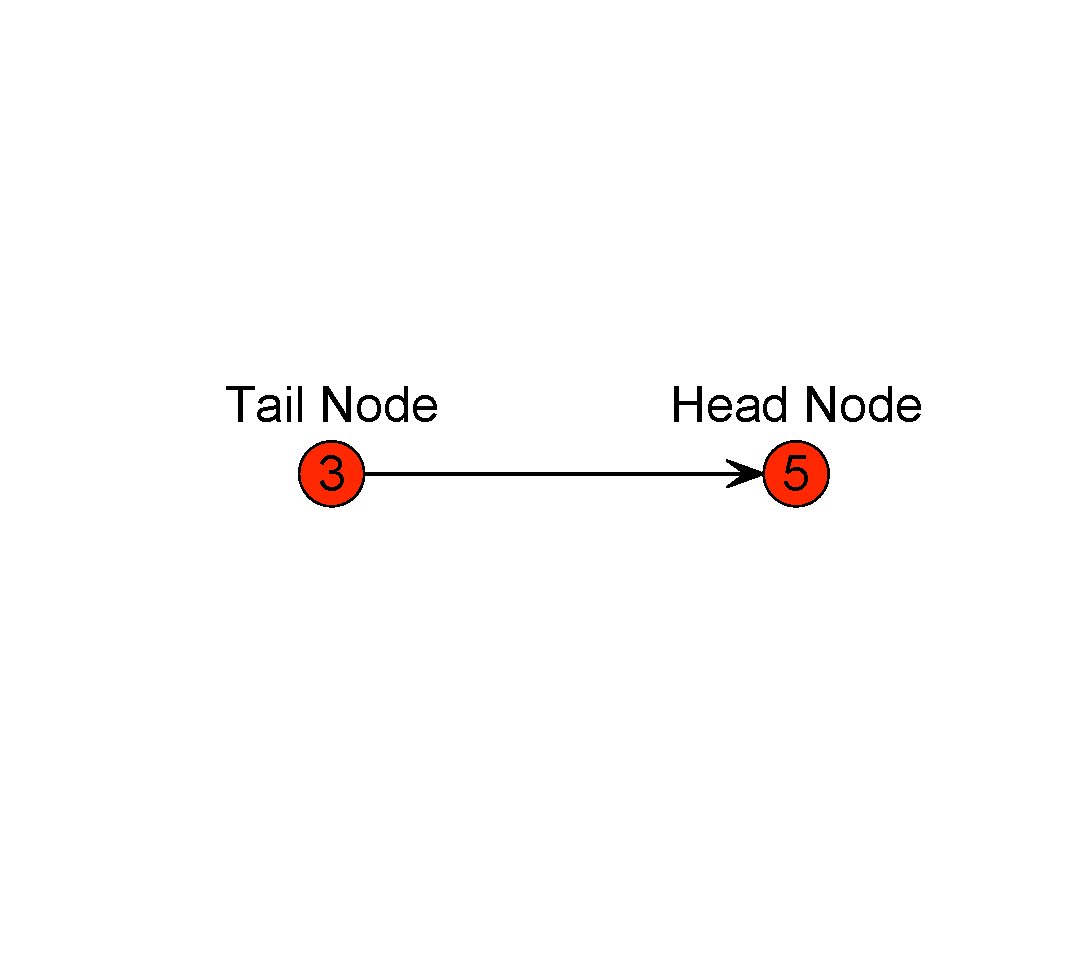
\includegraphics[width=3in]{twonode.pdf}}
\caption{A directed edge, sometimes termed an arc, from
node 3 to node 5.}\label{directededge}
\end{figure}

A network
with $n$ nodes is internally represented in \pkg{ergm} as a set of $2n$ edgelists,
$n$ for ``in-edges'' and $n$ for ``out-edges''.  If the directed edge
$3\!\!\longrightarrow\!\!5$ exists in the network,
then we call 3 the ``tail'' node and 5 the ``head'' node of this edge.  We would say node 3 
has an {\em out-edge} to node 5 and that node 5 has an {\em in-edge} from node 3, as depicted in
Figure~\ref{directededge}.  Thus, the 3rd out-edge list
should contain 5 and the 5th in-edge list should contain 3.  This redundant storage
scheme, requiring double the memory that a single representation of the network
would require, results in a corresponding gain in efficiency, since every edge
may be accessed via either of its nodes.

Undirected networks are effectively stored as directed networks in \pkg{ergm}
but with the ``directed'' flag set to zero rather than one.  Essentially, this means that
the adjacency matrix of an undirected network is represented as having only zeros
below the main diagonal; the ``tail'' node is taken to be the lower-numbered node
in each undirected node pair.  
For example, the undirected edge
$2\!\!\longleftrightarrow\!\!4$ would actually be stored as the directed edge
$2\!\!\longrightarrow\!\!4$.  Every routine written to handle undirected networks
must therefore check that the directed flag is set to zero and that every edge is
referenced as $\mbox{tail}\longrightarrow\mbox{head}$ where
$\mbox{tail}<\mbox{head}$.

\begin{figure}[htb]
\centerline{\vspace{3ex}
$\displaystyle{\pmatrix{
 0 & 0 & 1 & 0 & 0 & 1 & 0 & 1 \cr
 0 & 0 & 0 & 0 & 1 & 0 & 0 & 0 \cr
 0 & 0 & 0 & 0 & 0 & 1 & 1 & 1 \cr
 0 & 1 & 0 & 0 & 1 & 0 & 1 & 0 \cr
 1 & 1 & 1 & 1 & 0 & 0 & 0 & 0 \cr
 1 & 1 & 0 & 0 & 0 & 0 & 0 & 1 \cr
 0 & 0 & 0 & 0 & 0 & 0 & 0 & 0 \cr
 1 & 0 & 1 & 0 & 1 & 0 & 0 & 0 }
 }\qquad\qquad\vtop{\vskip-12ex \hbox{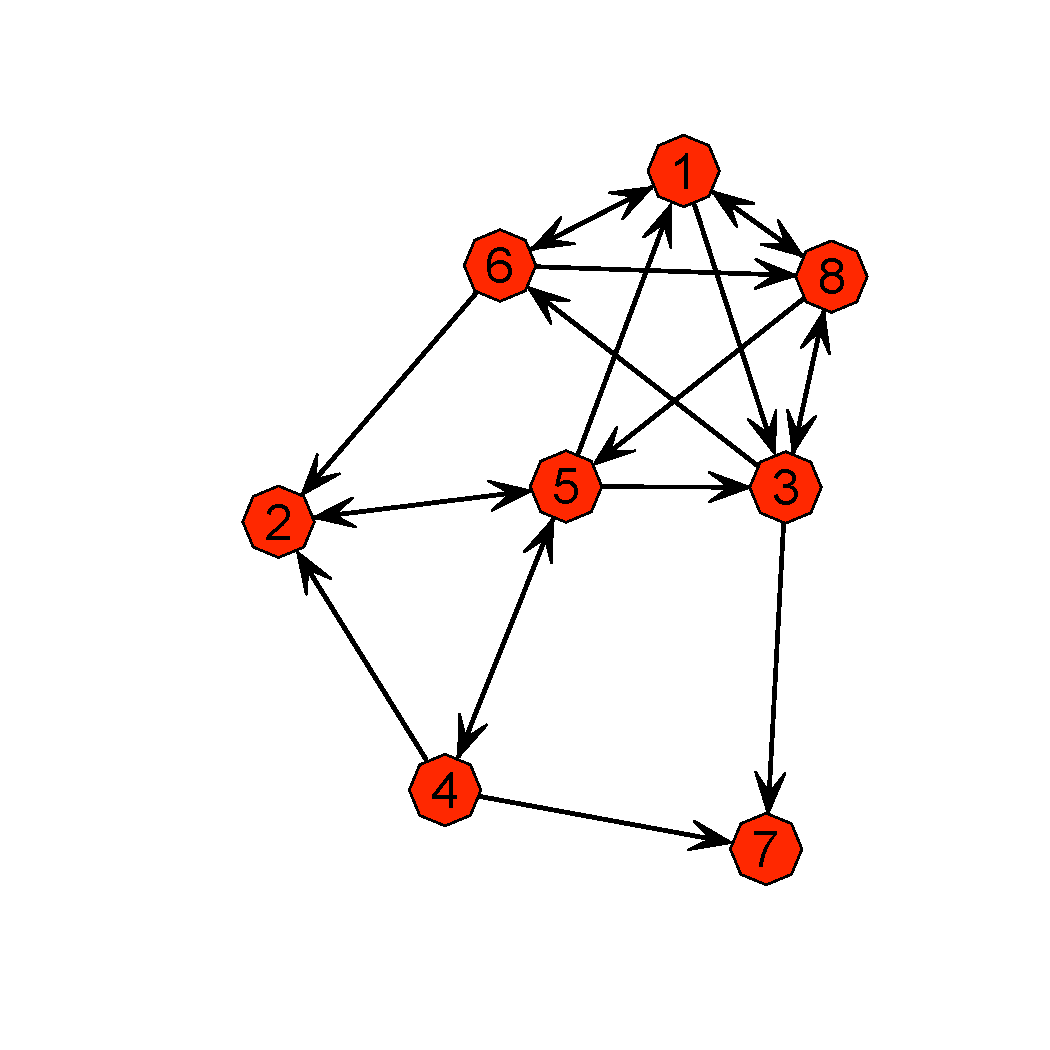
\includegraphics[height=1.75in, width=1.75in]{net8nodes.pdf}}}
$}
\caption{Adjacency matrix (left) and corresponding graphical representation
of a directed 8-node network (right).  The rows of the adjacency matrix define
the out-edge lists of Figure~\ref{outedgefig}.}\label{8nodeexample}
\end{figure}

\begin{figure}[htb]
\centerline{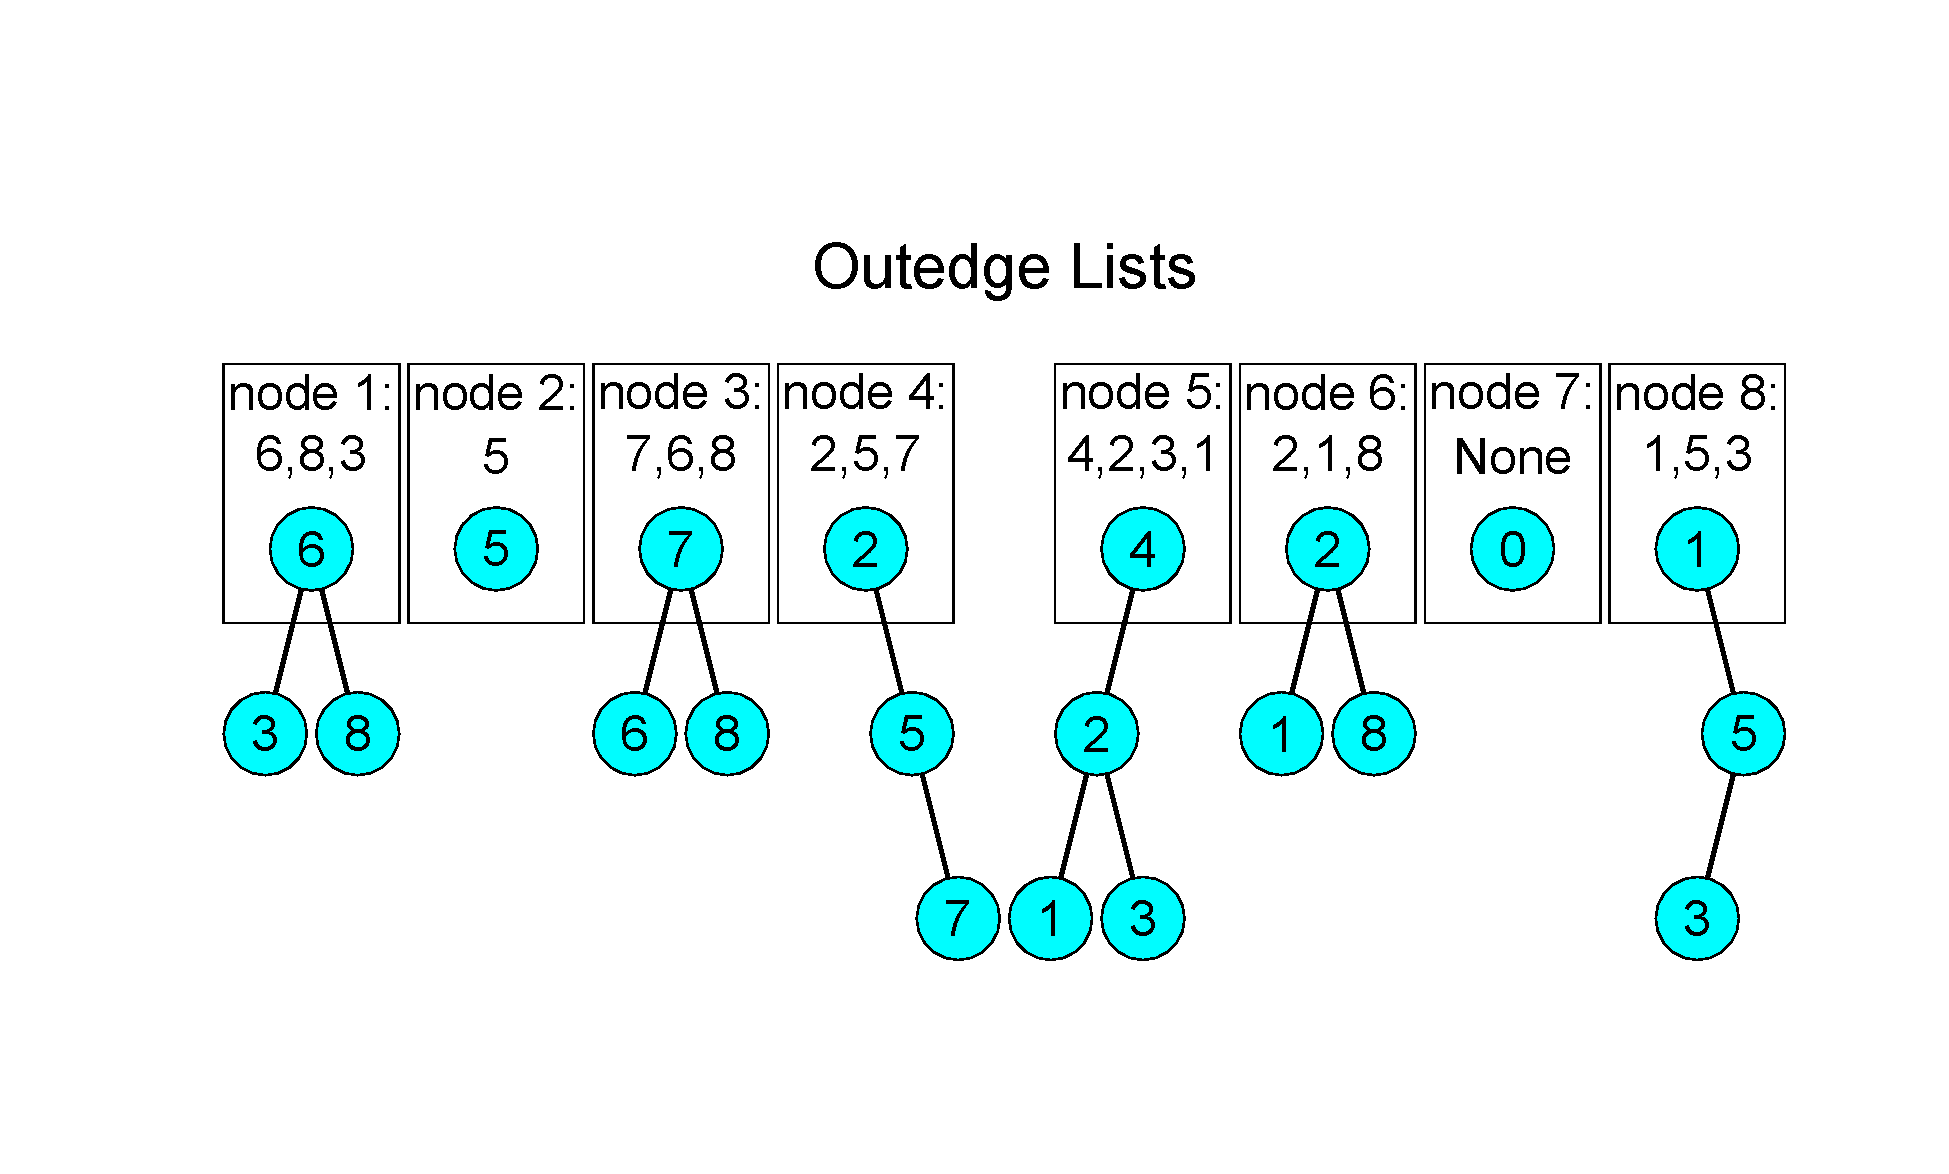
\includegraphics[height=2in, width=4in]{outedgelists.pdf}}
\caption{This is one possible \pkg{ergm} 
representation of the out-edges for the network of
Figure~\ref{8nodeexample}. The network would be redundantly represented as
a set of in-edge trees.}\label{outedgefig}
\end{figure}

Storage of each node's in-edge list and out-edge list is implemented using a
standard binary tree structure \citep[Chapter 13]{algorithms}. This 
structure allows for efficient lookup, insertion, and deletion operations that
typically take $O(\log d)$ time, where $d$ is the degree, or number of
neighbors, a particular node has. A set of binary trees representing the network of
Figure~\ref{8nodeexample} is given in Figure~\ref{outedgefig}. 
In this figure, every row of the adjacency matrix in Figure~\ref{8nodeexample}
is represented by its own tree, indexed by the tail node, where each numbered 
circular dot represents the head in a $(\mbox{tail}, \mbox{head})$ network edge.
Even the root of the tree is a head node, so in case the tail has no edges, the
root of the (empty) tree would have label 0.
Though the depiction of the trees in Figure~\ref{outedgefig} has its own network-like
appearance, this structure has nothing to do with the original network;
each tree is merely an efficient storage tool for a list of node labels.  In the trees,
each node may have up to two 
``child'' nodes, shown below it, one to the left and one to the right.
The rule for constructing the tree, which enables the fast lookup, insertion, and
deletion operations of a binary tree,
 is that the left child's label (if that child exists)
 must always be smaller than its parent's label while the
 right child's label must always be larger.
The designation of the root node's value in each tree is completely 
arbitrary, as a particular list of node labels might be used to populate
a tree in any order desired.
To avoid the worst-case performance that can result from a list
of values being passed in strictly increasing or decreasing order, each node's
edgelist is randomly permuted before it is stored as a tree.

The binary tree routines, all written in the \proglang{C} language, are contained in the
\code{src/edgetree.c} file in the \pkg{ergm.userterms} package. The \pkg{ergm} package
includes the same code.  These routines may be used to initialize or destroy
a network object, to manipulate that object by adding or deleting edges, and to
query that object to ascertain the presence of an edge.
The \proglang{C} language functions \code{NetworkInitialize} and \code{NetworkDestroy} 
are used internally by the \pkg{ergm} package to create a network object
and destroy it when it is no longer needed by the \proglang{C} code.  
These two functions
are not generally called by the user, though interested users may wish
to look at them.  Also, the definition of the \code{Network} type, in the
\code{src/edgetree.h} file, reveals that a network keeps updated lists of every node's
in- and out-degree in addition to the actual edges.  A user may exploit these statistics
when writing code for various change statistics as described in Section \ref{Cside}.

\section{Acquiring and setting up the necessary tools}
\label{Tools}

Coding new change statistics for \pkg{ergm} requires two steps that users might
not have previously encountered: building an \proglang{R} package from source,
and writing and compiling \proglang{C} code. These steps requires additional
tools beyond those needed by most \proglang{R} end users; in this section we
walk through the process of acquiring and setting up such tools in Windows or
UNIX-like operating systems (e.g., MacOS and Linux), with the emphasis on
Windows. 
Those users who are already familiar with this task may wish to skip ahead to
Section~\ref{Rside}.

Windows users require a bit of preliminary setup for the building-from-source
step, which we describe in the separate Section~\ref{AcqTools}.  Users of MacOS X
must install the \code{gcc}
compiler for \proglang{C}, which is found on the Xcode Tools CD or
DVD that accompanies the MacOS system.  Alternatively, the Xcode Tools may
be found in the \code{/Applications/Installers} directory or downloaded from the
web from \url{http://developer.apple.com/tools/xcode/}.  This is explained in the 
``Installation of source packages'' section of the
\proglang{R} MacOS X FAQ that may be reached from
\url{http://cran.r-project.org/faqs.html}.  Users of UNIX-like systems must merely
ensure that the \code{gcc} compiler is available, details of which may be
found at \url{gcc.gnu.org}.

\subsection{Setup for Windows}
\label{AcqTools}

Windows users will need three tools: Perl, CLT and MinGW.\footnote{This list of
necessary tools is current as of this writing. The authoritative and up-to-date
source for the set of tools necessary is Appendix D (``The Windows Toolset'') of
the \proglang{R} Installation and Administration manual
(\url{http://cran.r-project.org/doc/manuals/R-admin.html\#The-Windows-toolset})}
The easiest way to acquire all three is through the website ``Building
\proglang{R} for Windows'' (currently at
\url{http://www.murdoch-sutherland.com/Rtools}), which also provides an
excellent overview of the process described in this section. Simply download the
latest version of \code{Rtools.exe} from this website and install.  While 
doing so, be sure to check ``Edit the system PATH''; allow it to edit your path
so that \code{c:\textbackslash Program Files\textbackslash Rtools\textbackslash
bin}, \code{c:\textbackslash Program Files\textbackslash Rtools\textbackslash
perl\textbackslash bin}, and \code{c:\textbackslash Program Files\textbackslash
Rtools\textbackslash MinGW\textbackslash bin} are up front. After these three
entries, insert an additional entry containing the bin directory of your current
\proglang{R} installation. This is typically \code{C:\textbackslash Program
Files\textbackslash R\textbackslash R-X\textbackslash bin}, where \code{X} is
your \proglang{R} version number.


\subsection[Obtaining source code for the ergm.userterms package]{Obtaining source code for the \pkg{ergm.userterms} package}
\label{Source}

When one is planning only to use an \proglang{R} contributed package as-is and
not edit the source code, one need only install and load it using the \code{install.package} and \code{library} commands, respectively.
When wishes to edit the content, one must download the source code,
and then build from there. For all operating systems, one should:

\begin{enumerate}
\item Go to \url{www.r-project.org}, click on the CRAN link in the left-hand margin,
select a nearby mirror site, and finally click on the ``contributed extension packages''
link.
\item Select \pkg{ergm.userterms}.
\item Select the source code file (with extension \code{tar.gz}) next to ``Package Source''.
\item Save this file in \code{R-working-directory\textbackslash src\textbackslash library}.  Be very careful not to place it in \code{R-working-directory\textbackslash library}. In fact, you can technically place the file anywhere on your machine, as long as it is not in \code{R-working-directory\textbackslash library}.  In Windows, your \proglang{R} working directory will typically be \code{C:\textbackslash Program Files\textbackslash R\textbackslash R-X}, where \code{X} is your \proglang{R} version number).
\item Untar the file by opening a DOS window in
Windows (\code{Start>Run} and type \code{cmd}) or a terminal window in
UNIX-like systems,
navigating to the folder where you just saved the source code file
using \code{cd}, and typing \code{tar xfz name.of.sourcecode.file}.
A directory named \code{ergm.userterms} will be extracted in your current directory.
\end{enumerate}

\subsection[Building ergm.userterms]{Building \pkg{ergm.userterms}}
\label{BuildEUT}

For Windows, in a DOS window, go to the same directory where you saved the \pkg{ergm.userterms} source file in the previous step and type:
\begin{CodeChunk}
\begin{CodeInput}
RCMD INSTALL ergm.userterms
\end{CodeInput}
\end{CodeChunk}
For UNIX-like systems, use the same syntax but split \code{RCMD}
into two words: \code{R CMD}.
You can now load the basic \pkg{ergm.userterms} package within \proglang{R} with the \code{library(ergm.userterms)} command.

In Sections~\ref{Rside} and~\ref{Cside} we will describe the process of editing the \proglang{R} and \proglang{C} code to make new statistics.  Any time you have made changes that you want to see incorporated into the version of \pkg{ergm.userterms} that you are using in \proglang{R}, simply repeat the instructions here in section~\ref{BuildEUT}.

\section[Writing change statistics using ergm.userterms:  The R side]%
{Writing change statistics using \pkg{ergm.userterms}:  The \proglang{R} side}
\label{Rside}

A typical call to the \code{ergm} function might look like this:
\begin{CodeChunk}
\begin{CodeInput}
R> ergm ( network ~ edges + degree(1:3) + absdiff("age"))
\end{CodeInput}
\end{CodeChunk}
We refer to \code{edges}, \code{degree}, and \code{absdiff} as {\em terms}.
In the \pkg{ergm} package, there are roughly 70 terms available
as of this writing.
Documentation for these terms is
 in \citet{ergmtermsjss} and is also available by typing \code{help("ergm-terms")}.
 Terms may take arguments, such as the vector \code{1:3} or the nodal covariate
 name \code{"age"} above.  Implementing a new term that can be used by
 the \code{ergm} function involves adding two functions:  One written in \proglang{R}
 and one written in \proglang{C}.  This section describes the former, while Section \ref{Cside}
 describes the latter.

The \proglang{R} function, whose purpose is to initialize the internal representation
of the model term  just after a call to the  \code{ergm} function,
must be called \code{InitErgmTerm.termname}.  It should have a specified format and should
perform certain tasks.  We will examine these by considering the
\code{absdiff} term from the \pkg{ergm} package:
\begin{CodeChunk}
\begin{CodeInput}
 InitErgmTerm.absdiff <- function(nw, arglist, ...) {
  ### Check the network and arguments to make sure they are appropriate.
  a <- check.ErgmTerm(nw, arglist, directed=NULL, bipartite=NULL,
                      varnames = c("attrname","pow"),
                      vartypes = c("character","numeric"),
                      defaultvalues = list(NULL,1),
                      required = c(TRUE,FALSE))
  ### Process the arguments
  nodecov <- get.node.attr(nw, a$attrname)
  ### Construct the list to return
  list(name="absdiff",
       coef.names = paste(paste("absdiff", if(a$pow != 1) a$pow else "",
         sep = ""), a$attrname, sep = "."),
       pkgname = "ergm.userterms",
       inputs = c(a$pow, nodecov),
       dependence = FALSE )
}
\end{CodeInput}
\end{CodeChunk}
The \code{absdiff} term has one required argument, called \code{attrname}, and
one optional argument, called \code{pow}.  This term will add to the
model a network statistic equal to
\[
\sum_{i,j} y_{ij} |X_i-X_j|^p,
\]
where $X_i$ and $X_j$ are the values of the nodal covariate named \code{attrname}
(and assumed already to be part of the network object specified in the
\code{ergm} function call) and $p$ is the value of \code{pow}.  By default, \code{pow}
is one.

We now examine the \code{InitErgmTerm.absdiff} function line by line:
\begin{itemize}
\item[Line 1:]
Any \code{InitErgmTerm} function must take three arguments:
\code{nw}, \code{arglist}, and \code{...}.  The first of these will be the network object, from
which any necessary information may be extracted.  The second, \code{arglist},
will be the list of arguments passed by the user of the term, if any.  Finally, the ellipsis (``\code{...}'')
is necessary primarily for backward compatibility, as some existing InitErgmTerm arguments may
be passed additional arguments, and without the ellipsis, this could generate an error message.
\item[Line 3:]
The call to the \code{check.ErgmTerm} function should be performed by every
\code{InitErgmTerm} function, and its result is typically given the name \code{a}.
The first two arguments to \code{check.ErgmTerm} are the network and argument list; these
should not be modified.  However, the \code{directed} and \code{bipartite} arguments may
be set to \code{TRUE} or \code{FALSE} if the term should only be applicable to the specified
types of networks.  (An error results if a term is not appropriate, for example, if a directed network
is used in a call with a term for which \code{directed=FALSE}.)  Leaving \code{directed=NULL}
and \code{bipartite=NULL} indicates that the term may be used on either directed or
undirected, either bipartite or unipartite networks. In short, the values of \code{FALSE}, \code{TRUE}, and \code{NULL} for the
argument \code{directed} indicate that the term can be used on only undirected, only directed, or both types
of networks, respectively.  Likewise for \code{bipartite}.
\item[Line 4:]  Each argument to a term  (whether required or optional) has a name, and these names are
specified by \code{varnames}.  The \code{check.ErgmTerm}
function will return a list in which each item is named corresponding to its varname.
In the example, the list will have items named \code{attrname} and \code{pow}.
In the case of a term with no arguments (such as \code{edges}), use
\code{varnames=NULL}.
\item[Line 5:] In this example, the argument \code{attrname} is of type
\code{character} and the argument \code{pow} is of type \code{numeric}.
\item[Lines 6 and 7:] The \code{attrname} argument is required; i.e., an error results
if the user does not specify this argument.  Therefore, the default \code{NULL} is
irrelevant.  However, since \code{pow} is not required, its value will be set to the
default of 1 whenever the user does not supply it.
\item[Line 9:] This line extracts a vector of nodal covariate
values from the network object.  The name of this covariate was passed in by the
user and is the character string called \code{attrname} in the list returned by the
\code{check.ErgmTerm} function.
\item[Line 11:]  Each \code{InitErgmTerm} function should return, upon exit,
a list whose items are all named.  Some names are required, and some
are optional.  A full list of these is given in the header of the \code{InitErgmTerm.users.R}
file in the \code{R} subdirectory of the \pkg{ergm.userterms} package.
The first named item shown here, \code{name}, is required.  It gives the name
of the \proglang{C} function (when ``\code{d_}'' is prepended) that will calculate the
change statistic(s) for this term; see Section \ref{Cside} for details.  In this case,
we know that the function \code{d_absdiff} will be responsible for this calculation.
\item [Line 12:]  The \code{coef.names} is another required element in the output
list (the only one other than \code{name}).  It should give a vector of names
for the statistic(s) that are to be added to the model by this term.  The present
example adds only a single statistic whose name contains
both \code{absdiff} and the name of the nodal attribute, along with the exponent
\code{pow} if it is not one.  The length of the vector of statistic names determines how
many statistics \pkg{ergm} will expect the term to add to the model.
\item [Line 14:]
The \code{pkgname} is the name of the \proglang{R} package in which the
\proglang{C} function that calculates change statistics can be found.  By default,
this is \pkg{ergm}, but for new terms defined in the \pkg{ergm.userterms} package
the default must be overridden.
\item [Line 15:]
The \code{inputs} vector includes any information from the network object (other than the values of the ties) that must be made available to the \proglang{C} function that calculates the change statistic.  Because \code{absdiff} relies on the values of a nodal covariate, these values must be included in this case. In addition, the value of the
\code{pow} exponent must be available.  All these values
are concatenated into a single numeric vector and given the name \code{inputs} in the
list. Although the order in which they are included is arbitrary, the single values and shorter vectors are typically placed before the nodal attribute vector in order to make the indexing easier when they are retrieved within the \pkg{C}.
\item[Line 16:]  The \code{dependence=FALSE} means that this term does not, by itself,
result in an ERGM in which the dyads are dependent.   If all terms in a model
have \code{dependence=FALSE} set, then the entire model is a dyadic independence
model.  By default, if \code{dependence} is omitted then it is assumed \code{TRUE}.
\end{itemize}
One additional item that can go
in the output list is \code{emptynwstats}, which is a vector of the
same length as the number of statistics generated by the term being added.  This vector
gives the value of the network statistic measured on a network with no edges.  The reason for
this is that the empty network gives a point of reference for calculating global values of the statistics using \proglang{C} code that only calculates change statistics.
By default, \code{emptynwstats} is a vector of zeros, so it is only necessary to include this
item for cases where the empty network does not have the value zero for some of the statistics.
For instance, the \code{isolates} term counts the number of zero-degree nodes in the network,
and this statistic equals $n$ when the network is empty; thus, the \code{InitErgmTerm.isolates}
function ends with the following lines:
\begin{CodeChunk}
\begin{CodeInput}
  list(name="isolates",
       coef.names = "isolates",
       emptynwstats = network.size(nw) )
\end{CodeInput}
\end{CodeChunk}

Other items that can go into the
output list are described in the comments at the top of the
\code{InitErgmTerm.users.R} file in the \code{R} subdirectory of the \pkg{ergm.userterms}
package.  Those not described above deal with curved exponential family models,
which we do not discuss here; nonetheless, the reader is encouraged to read the
comments at the top of the \code{InitErgmTerm.users.R} file.

Any \code{InitErgmTerm} function will be automatically included in the \pkg{ergm.userterms}
package if it is saved in a file ending with the extension \code{.R} in the \code{R} subdirectory.
For instance, a user may simply use a text editor to add new \code{InitErgmTerm}
functions to the existing \code{InitErgmTerm.users.R} file; these
functions will then automatically be incorporated into the \pkg{ergm.userterms}
package.  By analogy, the \code{InitErgmTerm.absdiff} function examined here is 
found in the \code{InitErgmTerm.R} file in the \code{R} subdirectory in the
\pkg{ergm} package; indeed, that file contains a wealth of other examples that
may be examined, copied, and modified by users interested in 
producing their own model terms.

\section[Writing change statistics using ergm.userterms:  The C side]%
{Writing change statistics using \pkg{ergm.userterms}:  The \proglang{C} side}
\label{Cside}

As explained at the beginning of Section \ref{Rside}, adding a term to be
used with the \pkg{ergm} package requires two different functions:  An
\code{InitErgmTerm} function written in \proglang{R} and a
change statistic function written in \proglang{C}.  This section discusses the
second of these, which should be placed in a file with the extension \code{.c}
in the \code{src} directory, just as the examples in the
\pkg{ergm.userterms} package are found in the \code{changestats.c}
file.
Any \code{.c} file placed in the \code{src} subdirectory in the
\pkg{ergm.userterms} package will
automatically be compiled when the package is installed from source. Just be sure to include the line:
\begin{CodeChunk}
\begin{CodeInput}
#include "changestat.h"
\end{CodeInput}
\end{CodeChunk}
at the beginning of the file.

Readers familiar with writing \proglang{C} code may at first not recognize
the example \code{d_absdiff} function shown below.  This is because it
uses numerous macros, named using all capitals
in the \code{changestat.h} file in the
\code{src} directory, that are designed to make writing change statistic
functions easier.
For instance, an author of the \code{absdiff} term need not worry about
the arguments that will be required of the \code{d_absdiff} function; these
are automatically included by typing
\code{CHANGESTAT_FN(d_absdiff)}.  Here, \code{CHANGESTAT_FN} is a macro
defined to create a new function whose name is supplied by the user and
whose arguments agree exactly with the arguments that will automatically be passed to
it by the \pkg{ergm} package.

Here, then, is the code for the \code{d_absdiff} statistic:
\begin{CodeChunk}
\begin{CodeInput}
CHANGESTAT_FN(d_absdiff) {
  double change, p; Vertex t, h; int i;
  ZERO_ALL_CHANGESTATS(i);
  FOR_EACH_TOGGLE(i) {
    t = TAIL(i); h = HEAD(i);
    p = INPUT_PARAM[0];
    if(p==1.0){
      change = fabs(INPUT_PARAM[t] - INPUT_PARAM[h]);
    }else{
      change = pow(fabs(INPUT_PARAM[t] - INPUT_PARAM[h]), p);
    }
    CHANGE_STAT[0] += IS_OUTEDGE(t,h) ? -change : change;
    TOGGLE_IF_MORE_TO_COME(i); /* Needed in case of multiple toggles */
  }
  UNDO_PREVIOUS_TOGGLES(i); /* Needed on exit in case of multiple toggles */
}
\end{CodeInput}
\end{CodeChunk}
Following the first line, various variables are declared.  The \code{Vertex} type
is a safe way to declare any integer variables that may be as large as the total number of
vertices in the network; there is also a similar \code{Edge} type.
After the variable declarations, essentially every change statistic function has the following
form:
\begin{CodeChunk}
\begin{CodeInput}
  ZERO_ALL_CHANGESTATS(i);
  FOR_EACH_TOGGLE(i) {
    /* body of function */
    TOGGLE_IF_MORE_TO_COME(i); /* Needed in case of multiple toggles */
  }
  UNDO_PREVIOUS_TOGGLES(i); /* Needed on exit in case of multiple toggles */
\end{CodeInput}
\end{CodeChunk}
The \code{body} of the change statistic function has the goal of
updating the \code{CHANGE_STAT} vector, which has entries
\code{CHANGE_STAT[0]}, \ldots,
\code{CHANGE_STAT[N_CHANGE_STATS-1]},
as appropriate for the $i$th toggle specified by
\code{TAIL(i)}, \code{HEAD(i)}.  It is this portion of the function that should
be changed according to the requirements of the model statistic(s) specified by 
the term in question.  

Here, we briefly describe the logic of the code, consisting completely of
pre-defined macros, surrounding the \code{body} of the change statistic function.
However, it is not actually necessary to understand this logic thoroughly in order to
write change statistics functions; simply copy the syntax above.
The Metropolis-Hastings proposal could possibly involve
multiple edge toggles, and the job of the change statistic function is to update the
change statistics as appropriate for the entire set of toggles.
Since some of the macros, such as \code{ZERO_ALL_CHANGESTATS} and
\code{FOR_EACH_TOGGLE},
 require the use of a variable (such as \code{i} in the code above), it is important
 that this variable be declared as type \code{int} prior to its first use.

Inside the \code{FOR_EACH_TOGGLE(i)} loop, the value of \code{i}
counts from 0 to \code{ntoggles-1}, where \code{ntoggles} is the total number of
toggles being considered.  In each case, the proposed toggle---from edge to non-edge
or vice-versa, depending on the current state---is to the
ordered node pair (\code{TAIL(i), HEAD(i)}).  
Even when the network is considered undirected,
every edge is stored as a directed edge from the ``tail'' node to the ``head'' node.
After initially zeroing all of the change statistics using the
\code{ZERO_ALL_CHANGESTATS} macro, the function should, for each edge
toggle proposed, calculate how the toggle would change the network statistics of the
network.  This is a subtle difference here as compared to  the $\delta(y)_{th}$ function of
Equation~(\ref{changestats}), where the change is always calculated as the edge $(t,h)$
changes from 0 to 1.  In a change statistic function in \pkg{ergm}, however, the sign of the
change will depend on whether the proposed toggle is to an existing edge or not.

We may see how this is done by examining the body of the \code{d_absdiff} function below.
Remember that \code{t} and \code{h} are variables of type \code{Vertex} (which is essentially
the same as type \code{int}), whereas \code{p} and \code{change} are of type
\code{double}:
\begin{CodeChunk}
\begin{CodeInput}
    t = TAIL(i); h = HEAD(i);
    p = INPUT_PARAM[0];
    if(p==1.0){
      change = fabs(INPUT_PARAM[t] - INPUT_PARAM[h]);
    }else{
      change = pow(fabs(INPUT_PARAM[t] - INPUT_PARAM[h]), p);
    }
    CHANGE_STAT[0] += IS_OUTEDGE(t,h) ? -change : change;
\end{CodeInput}
\end{CodeChunk}
The first step in the body of our change statistic function is to read the value of
the exponent, determine whether or not it equals one, and act
accordingly.  
When the \code{inputs} vector was added to the output list of the
\code{InitErgmTerm.absdiff} function, it consisted of the exponent
followed by the values of some nodal attribute, one
for each of the $n$ nodes.  All of these inputs may be accessed now as the
elements of the \code{INPUT_PARAMS} vector, which has entries
\code{INPUT_PARAMS[0]} through \code{INPUT_PARAMS[N_INPUT_PARAMS-1]}.
Thus, the exponent may be read as
\code{INPUT_PARAM[0]}, which is why the code above sets \code{p} to this value.
It then calculates the absolute value of the
difference of the nodal attributes for the nodes numbered \code{t} and \code{h},
for these are the nodes involved in the proposed toggle.  If necessary (i.e.,
if \code{p} is not one),
the absolute difference is raised to the appropriate power.
The change statistic---there is only one change statistic,
\code{CHANGE_STAT[0]}, in this case---will then be equal to plus or minus
the exponentiated absolute difference, depending on the value
returned by the \code{IS_OUTEDGE} macro.  In Section \ref{networkstorage},
we explained that each node's full list of in-edges and out-edges is constantly
updated.  Therefore, each edge is listed in two places, so that if the
edge \code{(t,h)} is currently in the network, both
\code{IS_OUTEDGE(t,h)} and \code{IS_INEDGE(h,t)} would return one
rather than zero.\footnote{This is not the same as saying that
both \code{IS\_OUTEDGE(t,h)} and \code{IS\_INEDGE(t,h)} would return one rather than zero.  This is particularly true for undirected networks, where the edge
$t\!\longleftrightarrow\!h$ is always stored as
$t\!\longrightarrow\!h$ where $t<h$, so
\code{IS\_INEDGE(t,h)} would {\em never} return one when $t<h$.}
In this case, it suffices to check whether \code{(t,h)} is
an outedge:  If it is, then the toggle would remove the edge and so
we should add \code{-change} to \code{CHANGE_STAT[0]}; otherwise,
we should add \code{change}.  Since each example in this
article involves a term for which 
\code{N_CHANGE_STATS} is equal to one, the reader might 
benefit from examining the \proglang{C}
code for a term in the \pkg{ergm} package that can involve
more than one change statistic, such as 
\code{degree} or \code{nodematch}.

In some change statistic functions, it is necessary to look at all of the current
neighbors of a particular node.  The macros
\code{STEP_THROUGH_OUTEDGES} and \code{STEP_THROUGH_INEDGES}
can help with this.  Each of these macros takes three arguments; suppose
we call them $(a, e, v)$.  The first argument (which should be declared to of type \code{Vertex}) is the node whose in- or out-edges
we wish to examine.  The second argument (of type \code{Edge}) is the looping
variable that steps through each of the neighbors of \code{a} in turn.  Finally,
the third variable (of type \code{Vertex}) is set by the macro to equal the number of
the node corresponding to the edge.  It is important to remember that for undirected
networks, each edge is only stored as $(t,h)$, where $t<h$.
Therefore, to step
through all of the edges of node \code{t} in an undirected network, it is necessary
to step through all of its in- and out-edges by using
\code{STEP_THROUGH_OUTEDGES(t, e, v)}
followed by
\code{STEP_THROUGH_INEDGES(t, e, v)}.  It is possible to observe
examples of these macros in the \code{changestats.c} file in the
\pkg{ergm} package.

Other macros are described briefly in the file \code{changestat.h} in the \code{src}
directory.  Again, many examples of the use of these macros are available in the
\code{changestats.c} file.


\section{Worked example: a term for ``minimum degree''}
\label{Example}

Degree distributions are of interest in many social network applications, and the \pkg{ergm} package
includes a variety of terms to model the propensities for nodes to display different degrees or degree distributions.  The most straightforward is the \code{degree} term, which takes an argument comprising a vector of non-negative integers. The term returns a statistic for each element in the vector, representing the number of nodes whose degree equals exactly that element.  The \code{gwd} term provides one parsimonious method for capturing certain features of the degree distribution; however, one might reasonably be interested in specifying other aspects, such as the number of nodes of {\em at least} degree \code{n}, or of {\em no more than} degree \code{n}. The former may be useful, for instance, in testing the hypothesis that there is some social norm against having more than one alter, but that once one has two alters, there is no added propensity for or against acquiring additional ones. In this case, we would want to know whether we observe fewer nodes with degree of 2+ in our network than we would otherwise expect, and whether this model does a good job of fitting our data.  Let us define a new \pkg{ergm} term called \code{mindegree} to allow us to do this.

First, to the \proglang{R} side, where we must add a function called \code{InitErgmTerm.mindegree}.  We can do so either in the existing \code{InitErgmTerm.users.R} file, or in another file with extension \code{.R} that we create in the \code{R} directory of the \pkg{ergm.userterms} source code. To begin, we simply define the function and its arguments, remembering the standard set of arguments that we learned in Section~\ref{Rside} all such functions must have:
\begin{CodeChunk}
\begin{CodeInput}
InitErgmTerm.mindegree <- function(nw, arglist, ...) {
  # More lines coming....
}
\end{CodeInput}
\end{CodeChunk}

Next, we must add the call to \code{check.ErgmTerm}, where we may specify
whether we want this statistic to be usable for undirected networks,
directed networks, or both, and also whether it should be usable for bipartite networks.
The existing \pkg{ergm} term \code{degree} is limited to undirected networks, with \code{idegree} and \code{odegree} used to capture the two types of degree (in-degree and out-degree, respectively) for directed networks. Thus, it seems most reasonable for us to limit mindegree to undirected networks as well; users interested in analogous statistics for directed networks might choose to code up statistics called, for example, \code{min.idegree} and \code{min.odegree}. Likewise, bipartite networks will typically require separate degree terms for each of the two modes of the network.
Filling in our progress so far yields:
\begin{CodeChunk}
\begin{CodeInput}
InitErgmTerm.mindegree <- function(nw, arglist, ...) {
  a <- check.ErgmTerm(nw, arglist, directed=FALSE, bipartite=FALSE,
    # More args to check.ErgmTerm coming....
  # More lines coming....
}
\end{CodeInput}
\end{CodeChunk}
Next we must decide on the arguments for \code{mindegree}.  Certainly we must include at least one argument, the minimum degree.  The \code{degree} term also allows the user to specify, via the \code{by} argument, a nodal attribute on which ego and alter must match in order to be counted. 
For the sake of demonstration, we shall follow suit.  The \code{degree} term also has a \code{homophily}
argument, whose value is either \code{TRUE} or \code{FALSE}, and when it is
\code{FALSE} the meaning of the \code{by} argument changes.  We will not
duplicate the \code{homophily} option in \code{mindegree},
which is to say we will fix it as \code{TRUE}.
Note also that the degree term allows users to pass a vector of degrees, not just a single one.  In this case, it seems less likely that a user would be interested in multiple mindegrees than in multiple degrees; we will leave this feature off, and require the first argument to be a single non-negative integer, rather than a vector of arbitrary length.  Note that users who are interested in having multiple minimum degree statistics in a single model still have the option of including multiple mindegree terms in their formula.

This leaves us with two arguments (let's call them ``mindeg'' and ``by''). These
are of types numeric and character, respectively; required and optional,
respectively; and should probably have no default values:
 \begin{CodeChunk}
\begin{CodeInput}
InitErgmTerm.mindegree <- function(nw, arglist, ...) {
  a <- check.ErgmTerm(nw, arglist, directed=FALSE, bipartite=FALSE,
          varnames = c("mindeg", "by"),
          vartypes = c("numeric", "character"),
          required = c(TRUE, FALSE),
          defaultvalues = list(NULL, NULL))
  # More lines coming....
}
\end{CodeInput}
\end{CodeChunk}

Our remaining task is to generate the list to be returned by the function,
including any processing of arguments required for that list. In our case, the
values of some of our entries will vary depending on whether we are using the
homogeneous version of the statistic (i.e. without a nodal attribute) or the
attribute-specific version. One of these is the vector of attribute values,
which is commonly assigned to a vector named ``nodecov'' (for ``nodal
covariate'', a synonym for nodal attribute), a convention we shall follow here.
If there is no attribute, then nodecov will need to be assigned some value to
indicate that. Our \proglang{C} coding task will also be made easier if we pass
a flag (which we will call \code{attrflag}) that tells the \proglang{C} whether
or not to expect nodal attribute values. Looking over the various items that
need to be included in the list returned by the function, we see one other that
should vary between the homogeneous and attribute-specific versions: the names
of the statistic and coefficient, assigned to variable \code{coef.names}. If we
follow the example of the \code{degree} term, for the homogeneous version we
will want these to be named \code{mindegree}{\it x}, where {\it x} is the degree
cutoff for the statistic; with an attribute, they should be named
\code{mindegree.attrname}{\it x}, where \code{attrname} is the name of the
attribute in the \code{by} argument. For example, if the degree cutoff is 2, we
want the terms to be named \code{mindegree2} and \code{mindegree.attrname2},
respectively. Determining the values of \code{attrflag}, \code{nodecov}, and
\code{coef.names} thus all begin with the same condition, so we can combine them
in a single \code{if} statement:
\begin{CodeChunk}
\begin{CodeInput}
  if (is.null(a$by)) {
    attrflag <- 0
    nodecov <- NULL
    coef.names <- paste("mindegree", a$mindeg, sep=""),
  } else {
    attrflag <- 1
    nodecov <- get.node.attr(nw, a$by)
    coef.names <- paste("mindegree.", a$by, a$mindeg, sep=""),
    u <- sort(unique(nodecov))
    nodecov <- match(nodecov,u)
  }
\end{CodeInput}
\end{CodeChunk}

For the attribute-matching case, the object \code{nodecov} contains a vector of the
values of that attribute for all the nodes following the call to \code{get.node.attr}.
Within the \pkg{statnet} suite,
nodal attributes can be either numeric or character-based. It will much easier
to write \proglang{R} code converting a character-based attribute into a numeric
than it will be to write \proglang{C} code that can handle either a numeric or
character vector. This is because it doesn't matter what the actual values of
the attribute are for individual nodes; all that affects our statistic is
whether any two nodes have the same value or not. We can simply determine all of
the unique values for the attribute in our network, assign each a numeric value
(based on its alphabetic position, typically), and then replace the nodes'
character-based attribute values with the new numeric ranks. In \proglang{R},
one example of code to do this is:
\begin{CodeChunk}
\begin{CodeInput}
    u <- sort(unique(nodecov))
    nodecov <- match(nodecov,u)
\end{CodeInput}
\end{CodeChunk}
which has the added benefit of handling an attribute that is passed in as
numeric as well.

Some elements of the list to be returned by the function are straightforward
(\code{names}, \code{pkgname}, \code{dependence}). We have already addressed
\code{coef.names}. In the \code{inputs} vector, we combine everything that the
\proglang{C} code will need to know the value of: \code{mindeg} as well as the
\code{attrflag} and \code{nodecov} objects we made in the previous step. For an
empty network, the value of the mindegree statistic depends on what our minimum
degree cut-off is; if the cutoff is 0, then the statistic is equal to the number
of nodes in the network; but if the cut-off is any positive integer, then the
statistic is 0. Thus, our final returned list is going to be:
\begin{CodeChunk}
\begin{CodeInput}
  list(name = "mindegree",
    coef.names = coef.names,
    pkgname = "ergm.userterms",
    inputs = c(attrflag, a$mindeg, nodecov),
    dependence = TRUE,
    emptynwstats = (a$mindeg == 0) * network.size(nw)
  )
\end{CodeInput}
\end{CodeChunk}

Note that the dependence argument is not strictly needed, since the default is
TRUE, but is included for the sake of completeness.

One additional task we may wish to add is some checks on the arguments that the
user has passed. For instance, since the first argument for \code{mindegree}
differs from that of \code{degree} (constrained to be a single numeric in the
first case; allowed to be a vector in the latter), we may want to check that the
user has followed whatever documentation we will write for the statistic, rather
than assuming it is exactly parallel to \code{degree}:
\begin{CodeChunk}
\begin{CodeInput}
  if(length(a$mindeg) > 1)
    stop("The argument mindeg to mindegree expected a vector of length ",
         "1, but received a vector of length ",length(a$mindeg))
\end{CodeInput}
\end{CodeChunk}

Putting this all together gives us our complete \proglang{R} code:
\begin{CodeChunk}
\begin{CodeInput}
InitErgmTerm.mindegree <- function(nw, arglist, ...) {
  a <- check.ErgmTerm(nw, arglist, directed=FALSE, bipartite=FALSE,
      varnames = c("mindeg", "by"),
      vartypes = c("numeric", "character"),
      required = c(TRUE, FALSE),
      defaultvalues = list(NULL, NULL))
  if(length(a$mindeg) > 1)
    stop("The argument mindeg to mindegree expected a vector of length ",
         "1, but received a vector of length ",length(a$mindeg))
  if (is.null(a$by)) {
    attrflag <- 0
    nodecov <- NULL
    coef.names <- paste("mindegree", a$mindeg, sep="")
  } else {
    attrflag <- 1
    nodecov <- get.node.attr(nw, a$by)
    coef.names <- paste("mindegree.", a$by, a$mindeg, sep="")
    u <- sort(unique(nodecov))
    nodecov <- match(nodecov,u)
  }
  list(name = "mindegree",
      coef.names = coef.names,
      pkgname = "ergm.userterms",
      inputs = c(attrflag, a$mindeg, nodecov),
      dependence = TRUE,
      emptynwstats = (a$mindeg == 0) * network.size(nw)
  )
}
\end{CodeInput}
\end{CodeChunk}

Let us now turn to the \proglang{C}. Here again, we can choose to add our code
to the existing file \code{changestats.c} in the \code{src} directory of the
\code{ergm.userterms} source code, or create a new file (with extension
\code{.c}) to place in the same directory. If we do the latter, we must be sure
to include the line \code{\#include "changestat.h"} at the top of the file.

Following Section~\ref{Cside}, we know that the basic structure of our
\proglang{C} code must be:
\begin{CodeChunk}
\begin{CodeInput}
CHANGESTAT_FN(d_mindegree) {
  /* declarations to go here */
  ZERO_ALL_CHANGESTATS(i);
  FOR_EACH_TOGGLE(i) {
    /* body of function */
    TOGGLE_IF_MORE_TO_COME(i); /* Needed in case of multiple toggles */
  }
  UNDO_PREVIOUS_TOGGLES(i); /* Needed on exit in case of multiple toggles */
}
\end{CodeInput}
\end{CodeChunk}

We will need to conduct a different analysis depending on whether
\code{attrflag} is 0 or 1, so we should first check this value. Remember that in
the \proglang{R} code we passed the arguments to the \proglang{C} (via the
\code{inputs} element) in the order: \code{attrflag}, \code{mindeg},
\code{nodecov}.
Remember also that, whereas
\proglang{R} indexes its vectors starting at position 1, \proglang{C} does so
starting at 0.  Thus:
\begin{CodeChunk}
\begin{CodeInput}
  attrflag = INPUT_PARAM[0];
  if(attrflag==0){
    /* homogeneous version */
  }else{
    /* nodal attribute-specific version */
  }
\end{CodeInput}
\end{CodeChunk}

The homogeneous case (\code{attrflag=0}) is easier, so let us take this first.
If we were to toggle $y_{ij}$, how might it change the number of nodes in the
network with at least \code{mindeg} ties? If $y_{ij}=0$ (that is, a tie
currently does not exist), then we will be adding a tie. In that case, if node
$i$ currently has exactly \code{mindeg}$-1$ ties, adding tie $y_{ij}$ will cause
$i$ to have \code{mindeg} ties, and the statistic increases by 1; likewise for
node $j$. If $y_{ij}=1$ (i.e., a tie currently exists), then toggling it removes
the tie; in this case, if node $i$ currently has exactly \code{mindeg} ties,
removing $y_{ij}$ drops them below our threshold, and our statistic decreases by
one; likewise, again, for $j$. Looking in the description of the macros in
\code{changestat.h}, we see that there are macros called \code{IN_DEG} and
\code{OUT_DEG} to check for the in-degree and out-degree of a node; since we are
dealing with undirected networks only, which (as mentioned earlier) are stored
as directed networks, we must check both. 
Thus:
\begin{CodeChunk}
\begin{CodeInput}
CHANGESTAT_FN(d_mindegree) {
  /* declarations to go here */
  ZERO_ALL_CHANGESTATS(i);
  FOR_EACH_TOGGLE(i) {
    t = TAIL(i); h = HEAD(i);
    attrflag = INPUT_PARAM[0];
    mindeg = INPUT_PARAM[1];
    if(attrflag==0){
      tdeg = IN_DEG[t]+OUT_DEG[t];
      hdeg = IN_DEG[h]+OUT_DEG[h];
      CHANGE_STAT[0] += IS_OUTEDGE(t,h) ?
        - (tdeg==mindeg) - (hdeg==mindeg) :
        (tdeg==mindeg-1) + (hdeg==mindeg-1);
    }else{
      /* nodal attribute-specific version */
    }
    TOGGLE_IF_MORE_TO_COME(i); /* Needed in case of multiple toggles */
  }
  UNDO_PREVIOUS_TOGGLES(i); /* Needed on exit in case of multiple toggles */
}
\end{CodeInput}
\end{CodeChunk}

For the version with the nodal attribute, we need to read the values of that attribute for both $i$ and $j$ and then for all of their alters.  Since we are only considering those ties in which both the actor and their alter have the same attribute value, we must first consider whether $i$ and $j$ have the same value.  If they do not, then toggling their tie either on or off will not change our statistic. If they do have the same attribute value, then we need to consider the number of ties each has to alters with the same attribute value. We then have the same conditions for changing the statistic, depending on whether the tie is being toggled on or toggled off. In order to determine the nodal attribute for each of the alters, we can use two macros found in \code{changestat.h} and described in Section~\ref{Cside}: \code{STEP_THROUGH_OUTEDGES} and \code{STEP_THROUGH_INEDGES}. The new code, to go inside the \code{else} statement, is thus:
\begin{CodeChunk}
\begin{CodeInput}
      t_nodecov = INPUT_PARAM[t+1];
      h_nodecov = INPUT_PARAM[h+1];
      if (t_nodecov == h_nodecov) {
        hdeg = 0;
        STEP_THROUGH_OUTEDGES(h, e, node3) { /* step through outedges of head */
          if(INPUT_PARAM[node3+1]==h_nodecov){++hdeg;}
        }
        STEP_THROUGH_INEDGES(h, e, node3) { /* step through inedges of head */
          if(INPUT_PARAM[node3+1]==h_nodecov){++hdeg;}
        }
        tdeg = 0;
        STEP_THROUGH_OUTEDGES(t, e, node3) { /* step through outedges of tail */
          if(INPUT_PARAM[node3+1]==t_nodecov){++tdeg;}
        }
        STEP_THROUGH_INEDGES(t, e, node3) { /* step through inedges of tail */
          if(INPUT_PARAM[node3+1]==t_nodecov){++tdeg;}
        }
        CHANGE_STAT[0] += IS_OUTEDGE(t,h) ?
          - (tdeg==mindeg) - (hdeg==mindeg) :
          (tdeg==mindeg-1) + (hdeg==mindeg-1);
      }else{
        CHANGE_STAT[0] = 0;
      }

\end{CodeInput}
\end{CodeChunk}
The $+1$ in each of the \code{INPUT_PARAM} indices is because the input vector
is indexed as 0=\code{attrflag}; 1=\code{mindeg}; 2 to \code{popsize+1} = nodal
attribute value for nodes 1 to \code{popsize}.

Declaring all of the variables that we ended up using, and putting it all
together, yields:
\begin{CodeChunk}
\begin{CodeInput}
CHANGESTAT_FN(d_mindegree) {
  Vertex t, h, node3;
  int i, mindeg, hdeg, tdeg;
  Edge e;
  int attrflag;
  double t_nodecov, h_nodecov;

  ZERO_ALL_CHANGESTATS(i);
  FOR_EACH_TOGGLE(i) {
    t = TAIL(i); h = HEAD(i);
    attrflag = INPUT_PARAM[0];
    mindeg = INPUT_PARAM[1];
    if(attrflag==0){
      hdeg = IN_DEG[h]+OUT_DEG[h];
      tdeg = IN_DEG[t]+OUT_DEG[t];
      CHANGE_STAT[0] += IS_OUTEDGE(t,h) ?
        - (tdeg==mindeg) - (hdeg==mindeg) :
        (tdeg==mindeg-1) + (hdeg==mindeg-1);
    }else{
      t_nodecov = INPUT_PARAM[t+1];
      h_nodecov = INPUT_PARAM[h+1];
      if (h_nodecov == t_nodecov) {
        hdeg = 0;
        STEP_THROUGH_OUTEDGES(h, e, node3) { /* step through outedges of head */
          if(INPUT_PARAM[node3+1]==h_nodecov){++hdeg;}
        }
        STEP_THROUGH_INEDGES(h, e, node3) { /* step through inedges of head */
          if(INPUT_PARAM[node3+1]==h_nodecov){++hdeg;}
        }
        tdeg = 0;
        STEP_THROUGH_OUTEDGES(t, e, node3) { /* step through outedges of tail */
          if(INPUT_PARAM[node3+1]==t_nodecov){++tdeg;}
        }
        STEP_THROUGH_INEDGES(t, e, node3) { /* step through inedges of tail */
          if(INPUT_PARAM[node3+1]==t_nodecov){++tdeg;}
        }
        CHANGE_STAT[0] += IS_OUTEDGE(t,h) ?
          - (tdeg==mindeg) - (hdeg==mindeg) :
          (tdeg==mindeg-1) + (hdeg==mindeg-1);
      }else{
        CHANGE_STAT[0] = 0;
      }
    }
    TOGGLE_IF_MORE_TO_COME(i); /* Needed in case of multiple toggles */
  }
  UNDO_PREVIOUS_TOGGLES(i); /* Needed on exit in case of multiple toggles */
}
\end{CodeInput}
\end{CodeChunk}
Once both the \proglang{C} and \proglang{R} files are completed, one need simply rebuild the package from source, following the instructions in Section~\ref{BuildEUT} and the new terms should appear.

We find that one useful way to test code for new statistics is by generating a wide variety of networks for which one knows the correct values of the statistic, and then using the command:
\begin{CodeChunk}
\begin{CodeInput}
summary(network ~ new.change.stat)
\end{CodeInput}
\end{CodeChunk}
to ensure that the code is calculating the correct values.

\section{Discussion}

This paper describes how to extend the exponential-family random graph modeling
capabilities of the \pkg{statnet} suite of packages by
explaining how users may use and modify the template package \pkg{ergm.userterms} to develop custom terms that can be ``plugged in" to \pkg{statnet}. These terms can then use the full capabilities of the \pkg{statnet} suite of packages.
These terms will be computed at the \proglang{C} level and operate at native speeds. In
addition, they will be able to use the parallel capabilities of \pkg{statnet}
without further changes. 
%The advantage of a plug-in architecture is that the
%package will be more portable and be able to take advantage of enhancements to
%the \pkg{statnet} suite. 
Finally, users may make the new terms
available to the \pkg{statnet} community, hence extending the analysis and
modeling capabilities of \pkg{statnet}.

Additional examples abound within the \code{changestats.c} file in the source
code; collectively these demonstrate the syntax for the other macros listed in
\code{changestat.h} and should answer most other questions for users. When
relying on existing network statistics code as examples, it is important to
remember the caveat that versions of \pkg{ergm} prior to 2.3 used different
methods; these are still allowed for backward compatibility, but modifying
individual snippets of code from them and interacting them with newer code may
cause problems.

The fact that the \pkg{ergm.userterms} package comes with a number of macros to
make the coding of change statistics easier does not preclude users from
writing their own macros to further streamline coding. For
instance, the lines of code that currently must appear at the beginning and end
of each statistic's \proglang{C} code could be incorporated into a macro. Macros
of this type will likely appear in a future version
of the \code{ergm.userterms} package, although their use will always remain
optional.

Additional questions may be posted to the listserv for the \pkg{statnet} users'
group, which readers are encouraged to join \citep{statnetusersgroup}.

\section*{Acknowledgments}

We would like to thank the \pkg{statnet} team, and in particular, Martina Morris, Carter
Butts, Pavel Krivitsky, and Ayn Leslie-Cook.

\bibliography{v24}

%\newpage

%\begin{appendix}


%\section[appendix]{Appendix}
%\label{appendix}

%\end{appendix}

\end{document}
